\documentclass[../TDON2_inter.tex]{subfiles}%

\begin{document}
\section[s]"2"{Interférences et écoute musicale}
\enonce{%
	\noindent
	\begin{minipage}{0.60\linewidth}
		La qualité de l'écoute musicale que l'on obtient avec une chaîne hi-fi
		dépend de la manière dont les enceintes sont disposées par rapport à
		l'auditaire. On dit qu'il faut absolument éviter la configuration représentée
		sur la figure~: présence d'un mur à une «~petite~» distance $D$ derrière
		l'auditaire.
	\end{minipage}
	\hfill
	\begin{minipage}{0.40\linewidth}
		\begin{center}
			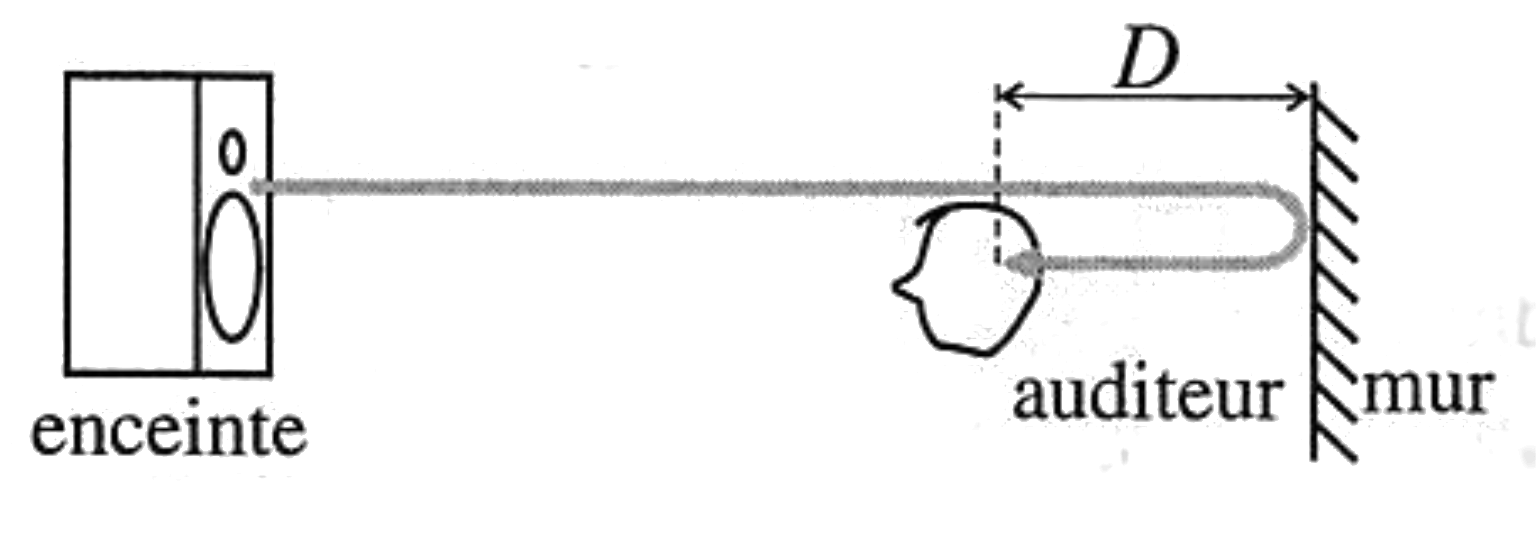
\includegraphics[width=\linewidth]{ecoute_musicale-plain_white}
		\end{center}
	\end{minipage}
	\bigbreak
	Comme représenté sur la figure, l'onde issue de l'enceinte se réfléchit
	sur le mur. On note $c = \SI{342}{m.s^{-1}}$ la célérité du son dans l'air.
}

\QR{%
	Exprimer le décalage temporel $\tau$ qui existe entre les deux ondes
	arrivant dans l'oreille de l'auditaire~: l'onde arrivant directement et
	l'onde réfléchie.
	\smallbreak
	En déduire le déphasage $\D\f$ de ces deux ondes supposées
	sinusoïdales de fréquence $f$. La réflexion sur le mur ne s'accompagne
	d'aucun déphasage pour la vibration acoustique.
}{%
	Chaque onde parcourt la distance enceinte -- auditaire directement,
	mais l'onde réfléchie parcourt en plus $2D$ entre l'auditaire et le mur.
	Ainsi, la célérité étant notée $c$, on a
	\[\tau = \frac{2D}{c}\]
	La source étant similaire pour les deux ondes, la phase à l'origine
	des temps est la même~; de plus il est indiqué que la réflexion
	sur le mur n'implique pas de déphasage supplémentaire, donc le déphasage
	n'est dû qu'à la propagation. Ainsi, l'onde réfléchie a un déphasage
	\[\D\f_{r/i}(\Mr) = \w\tau = \frac{4\pi fD}{c}\]
}

\QR{%
	Expliquer pourquoi il y a risque d'atténuation de l'amplitude de
	l'onde pour certaines fréquences. Exprimer ces fréquences en fonction
	d'un entier $n$. Quelle condition devrait vérifier $D$ pour qu'aucune de
	ces fréquences ne soit dans le domaine audible. Est-elle réalisable~?
}{%
	Il peut y avoir une atténuation de l'amplitude si les deux ondes sont
	en opposition de phase, et donc que les interférences sont destructives,
	c'est-à-dire
	\begin{gather*}
		\D\f_{r/i}(\Mr) = (2n+1)\pi
		\Lra
		\frac{4\cancel{\pi}f_nD}{c} = (2n+1)\cancel{\pi}
		\Lra
		\boxed{f_n = (2n+1) \frac{c}{4D}}
	\end{gather*}
	avec $n\in\Nb$. Étant donné que le domaine audible s'étant de
	$\SIrange{20}{20e3}{Hz}$, il faudrait que la plus petite fréquence
	d'atténuation, celle avec $n=0$, soit au-delà de \SI{20}{kHz}~;
	autrement dit on cherche
	\begin{gather*}
		f_{\max} < \frac{c}{4D}
		\Lra
		\boxed{D < \frac{c}{4f_{\max}}}
		\qavec
		\left\{
		\begin{array}{rcl}
			c        & = & \SI{342}{m.s^{-1}} \\
			f_{\max} & = & \SI{20}{kHz}
		\end{array}
		\right.\\
		\mathrm{A.N.~:}\quad
		\boxed{D < \SI{4.3}{mm}}
	\end{gather*}
	On est donc sûrx de ne pas avoir d'atténuation dans l'audible si on
	colle notre oreille au mur… ce qui est réalisable, mais correspond
	presque à ne pas avoir d'interférences du tout.
}

\QR{%
	Expliquer qualitativement pourquoi on évite l'effet nuisible en
	éloignant l'auditaire du mur.
}{%
	Quand $D$ augmente, l'onde réfléchie par le mur finit par avoir une
	amplitude faible devant l'onde directe étant donné qu'une onde sphérique
	voit son amplitude diminuer avec le rayon~: les interférences deviennent
	de plus en plus négligeables.
}
\end{document}
